\chapter{Results}\label{chap:5}

The six pairs organised their Tangram work through local attempts, suggestions, placements and revisions. Three connected findings emerged from the process records. First, a construction that resembled the target could conceal an unused piece or an incorrect proportion. Second, the division of work changed as participants encountered dependencies between parts of the construction. Third, an existing partial solution could be preserved by a partner and later revised by the person who had built it. Together, these findings connect the geometry visible in the workspace with the actions through which pairs developed and accepted a solution.

The analysis draws primarily on the researcher's video process records and the VR action and pose logs. Video records establish the sequence of proposals, responses and visible actions. Logs identify the manipulated pieces and record their positions, rotations, grabs and releases. The figures use these sources to show both the development of an arrangement and the people who changed it. Participants are identified by their P01--P12 codes throughout. Video timestamps locate events in a recording; active log seconds locate events within a research round.

\section{Plausible shapes and overlooked geometric problems}\label{sec:5-1}

In first-person VR, three of the six pairs produced a near-complete arrangement with an unused piece, or an arrangement using all seven pieces whose outline or proportions did not match the target. These were G01, G05 and G06. In the researcher's process records, none of the six pairs showed the same pattern in shared-overhead VR. The pattern concerns an arrangement that already resembled the target. Difficulty finding a solution, or having pieces left while a construction was still incomplete, was treated separately. Table~\ref{tab:5-1} shows how the three first-person cases developed and how their outcomes differed.

\par\addvspace{8pt}
\noindent\begin{minipage}{\linewidth}
\begingroup
\centering
\setstretch{1}
\fontsize{10}{12.3}\selectfont
\setlength{\tabcolsep}{2.2pt}
\renewcommand{\arraystretch}{1.18}
\captionof{table}[Near-complete shape problems in first-person VR.]{Near-complete shape problems in first-person VR. These are three cases within the six pairs, as identified in the researcher's process records.}\label{tab:5-1}
\begin{tabular}{@{}>{\raggedright\arraybackslash}p{16.614mm}>{\raggedright\arraybackslash}p{62.763mm}>{\raggedright\arraybackslash}p{77.531mm}@{}}
\toprule
\textbf{Pair} & \textbf{Problem in candidate} & \textbf{Response and outcome} \\
\midrule
G01 & Chair outline formed with the medium triangle unused. & Replacement was attempted and rejected when edges did not align. \\
\addlinespace[3pt]
G05 & All seven pieces formed a chair with an elongated proportion. & A partner questioned the result; revision continued. \\
\addlinespace[3pt]
G06 & Six-piece candle with the medium triangle unused, followed by rebuilding. & Seven-piece result accepted during the session; later reconstruction showed a proportion mismatch. \\
\bottomrule
\end{tabular}
\par\endgroup
\end{minipage}\par\addvspace{8pt}

G01 built a plausible chair outline while the medium triangle remained outside it. P02 brought the remaining piece to the partner's attention. The pair also adjusted access to the target: P01 lifted a large triangle to see the reference, and the arrangement was moved to make space around the silhouette. They then tried substituting the medium triangle for a smaller piece. The edges did not align, and the attempt was rejected. The handling of the pieces therefore served different purposes within one sequence: exposing the reference, displaying a problem and testing a candidate solution. [\hyperlink{src:D04}{D04}]

G05 reached a seven-piece chair whose proportions were too long. A partner questioned its match with the target, and exploration continued. The subsequent construction involved changing the role of the parallelogram between the seat and backrest. G05 thus provides a case in which a plausible whole was questioned during the task. G01 rejected a candidate when the replacement failed, whereas G06 accepted a final configuration whose geometric problem was identified later. [\hyperlink{src:D10}{D10}]

\subsection{G06 from a six piece candidate to accepted completion}\label{sec:5-1-1}

G06's candle provides the clearest link between the construction process and the later geometry check. P11 initially worked mainly on the body, while P12 worked on the top. Six pieces formed a recognisable candle, leaving the medium triangle unused. The pair tried to incorporate it, opened the body and developed another internal arrangement. The medium triangle was eventually included, and both participants accepted the seven-piece result. The researcher also accepted it during the session. [\hyperlink{src:D14}{D14}]

\begin{figureunit}{5-1}
Figure~\ref{fig:5-1} reconstructs six stages from the recorded piece poses. At 45 active log seconds, six pieces formed the candidate and the medium triangle remained outside it. The 64-second state shows an attempt to use the medium triangle; the 83-second state shows the body opened. By 145 seconds, the arrangement included a new large-triangle anchor. The medium triangle had been incorporated by 184 seconds, and the 214-second state shows the seven-piece configuration accepted at the end of the process. These states make the changes to the construction visible alongside the researcher's account.

\par\begingroup
\centering
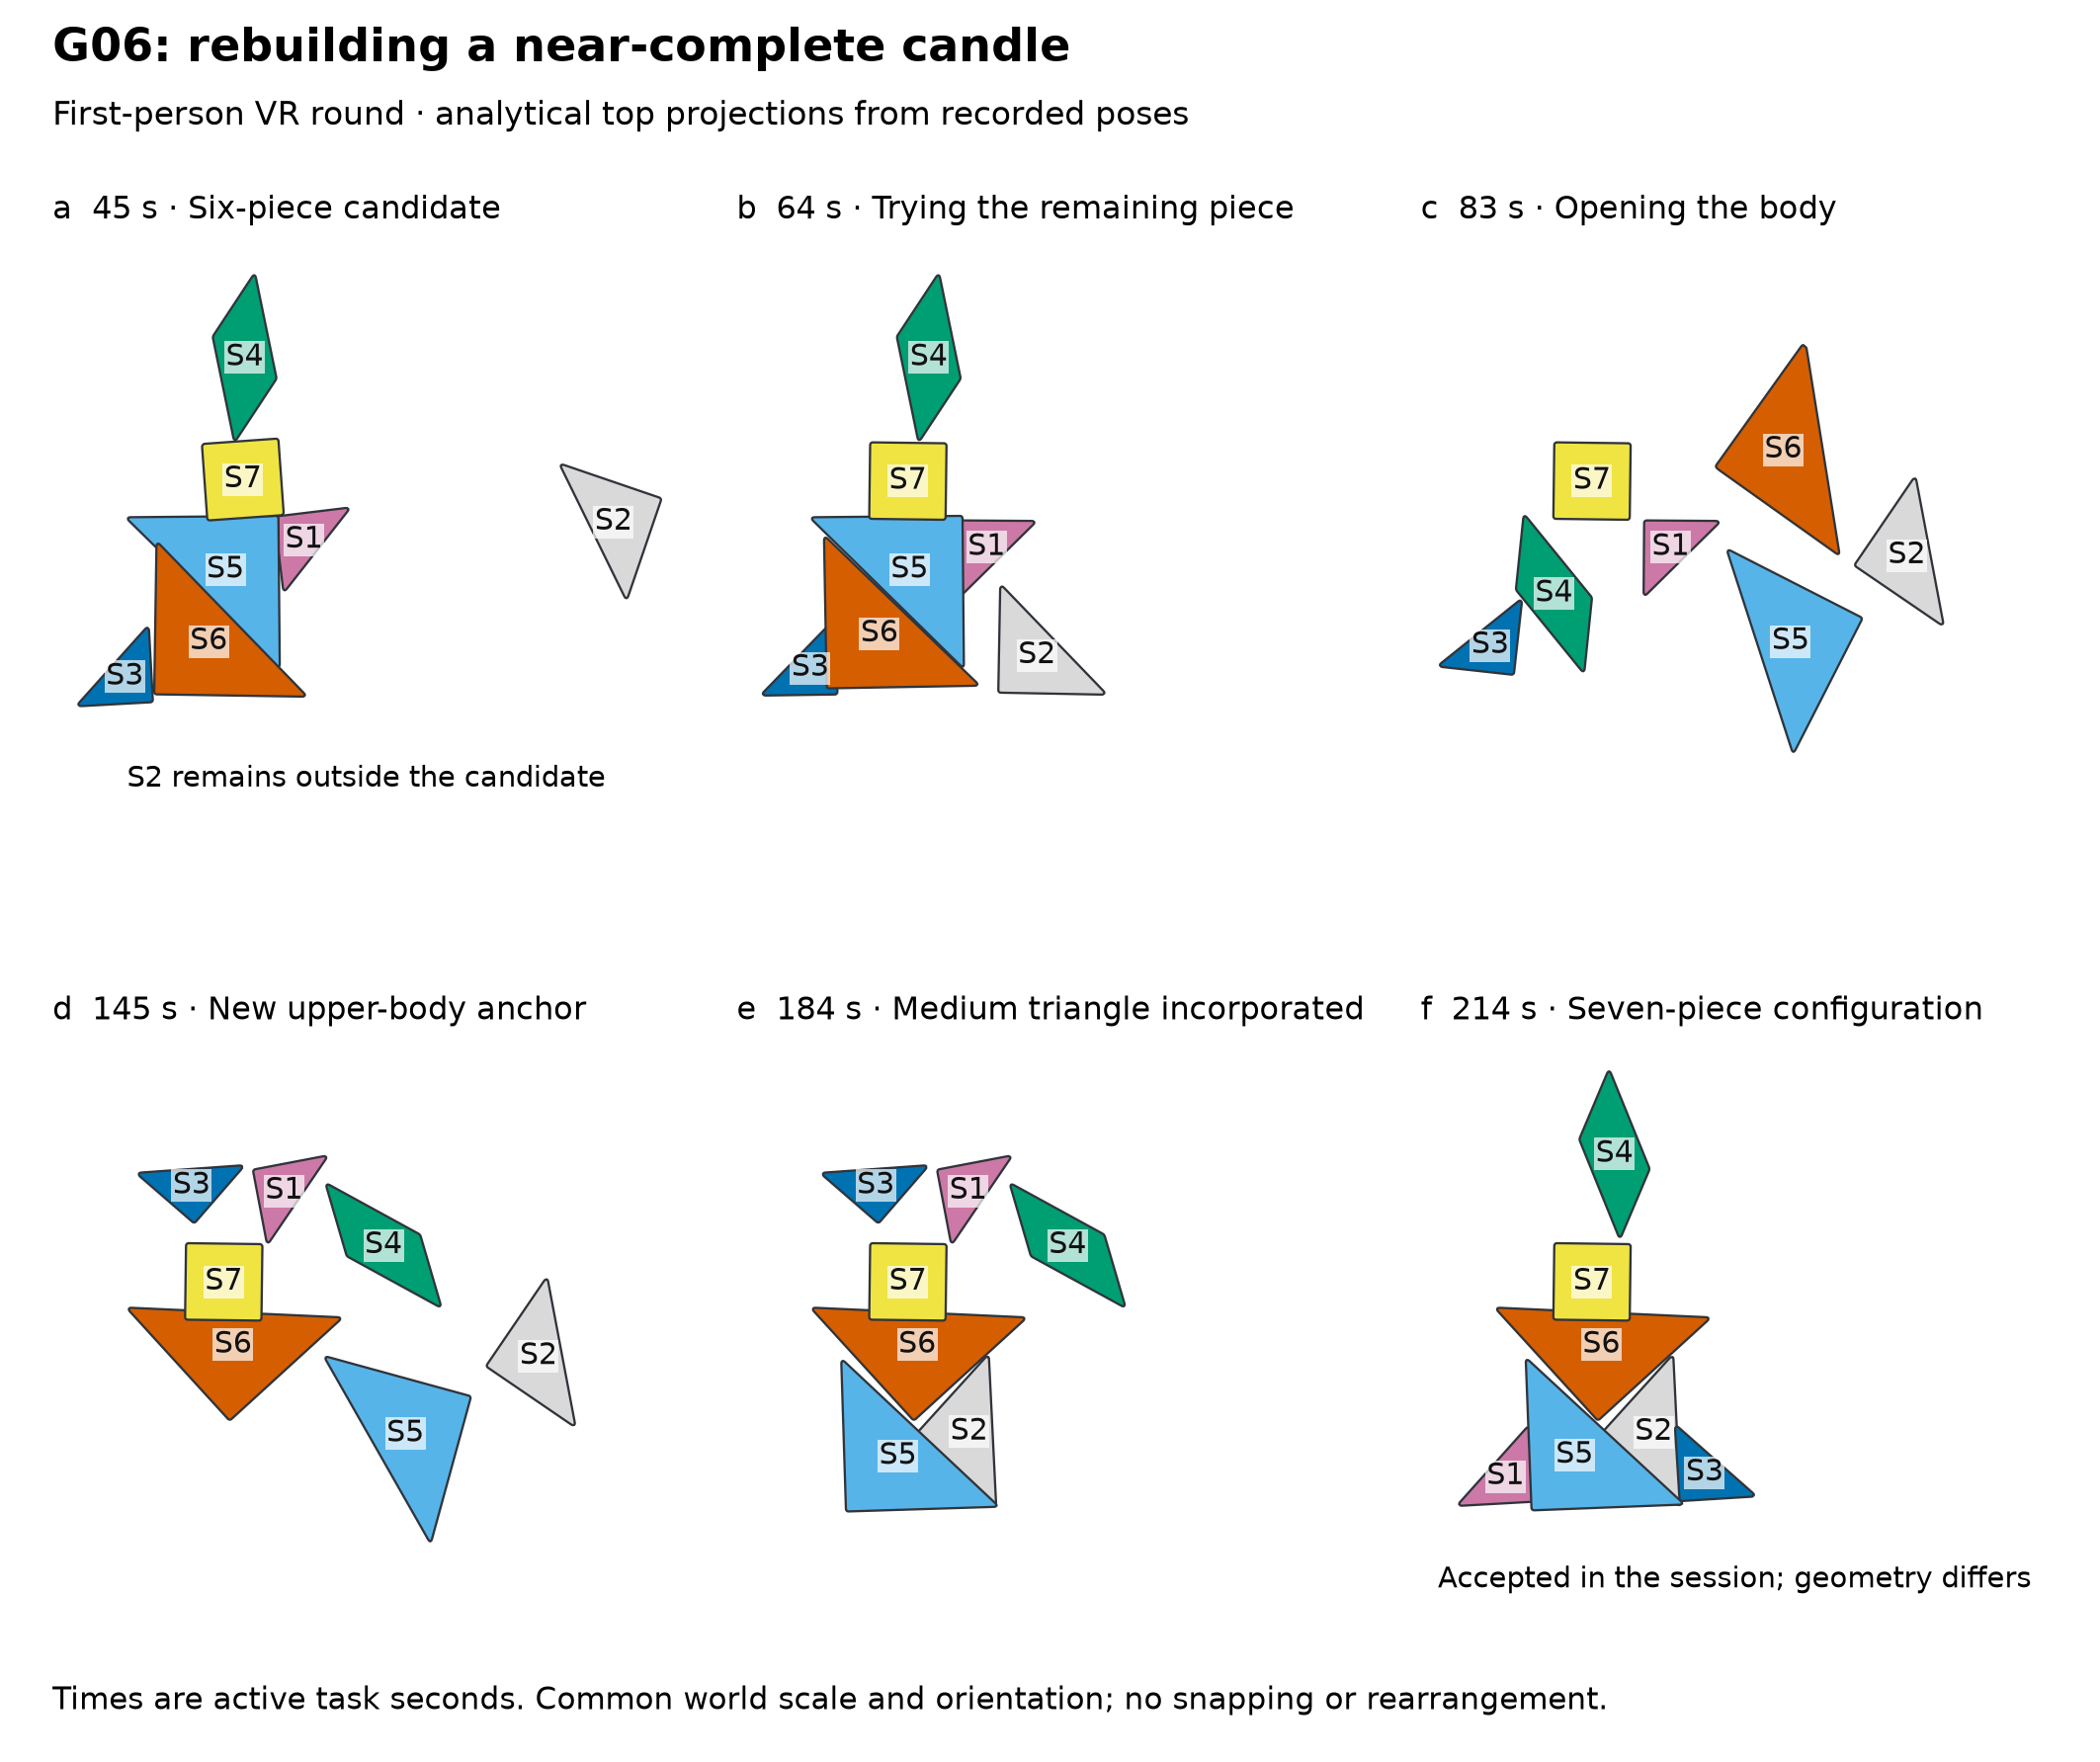
\includegraphics[width=\linewidth,height=134mm,keepaspectratio]{assets/figures/fig01_g06_reconstruction_sequence.png}
\captionof{figure}[G06's candle at six active-task times, reconstructed from the saved piece mesh and recorded poses.]{G06's candle at six active-task times, reconstructed from the saved piece mesh and recorded poses. Every panel has the same scale and world orientation. S2 is the medium triangle. No piece was snapped or rearranged. The video process record establishes acceptance of the final configuration; the logs establish the geometry. These analytical top projections were not participant views. The final outline is examined in Figures~\ref{fig:5-2} and~\ref{fig:5-3}. [\hyperlink{src:D14}{D14}]}\label{fig:5-1}
\par\endgroup
\end{figureunit}



While rebuilding the candle during the task, P11 asked to try another viewpoint, at approximately 13:46 in the available recording. View switching was locked during the formal round, so the pair continued in first-person VR. The request places viewing conditions within the participants' own efforts to resolve the task. The view remained first-person throughout the formal round. [\hyperlink{src:D14}{D14}]


\subsection{Reconstructing the accepted geometry}\label{sec:5-1-2}

\begin{figureunit}{5-2}
The researcher noticed that the accepted G06 candle was wider at the bottom than the target. Figure~\ref{fig:5-2} places the recorded first-person view beside the reconstruction, making the outline mismatch visible. Figure~\ref{fig:5-3} compares it with the target and two other first-person candle constructions. G03 and G04 use two equal large triangles for the corresponding upper and lower spans; G06 uses a different combination with a wider lower body. A supporting span comparison gives approximately 1.39 for G06 against 1.00 for the target and the other two constructions. These top views were reconstructed after the tasks to check the researcher's observation. [\hyperlink{src:D16}{D16}, \hyperlink{src:D74}{D74}]

\par\begingroup
\centering
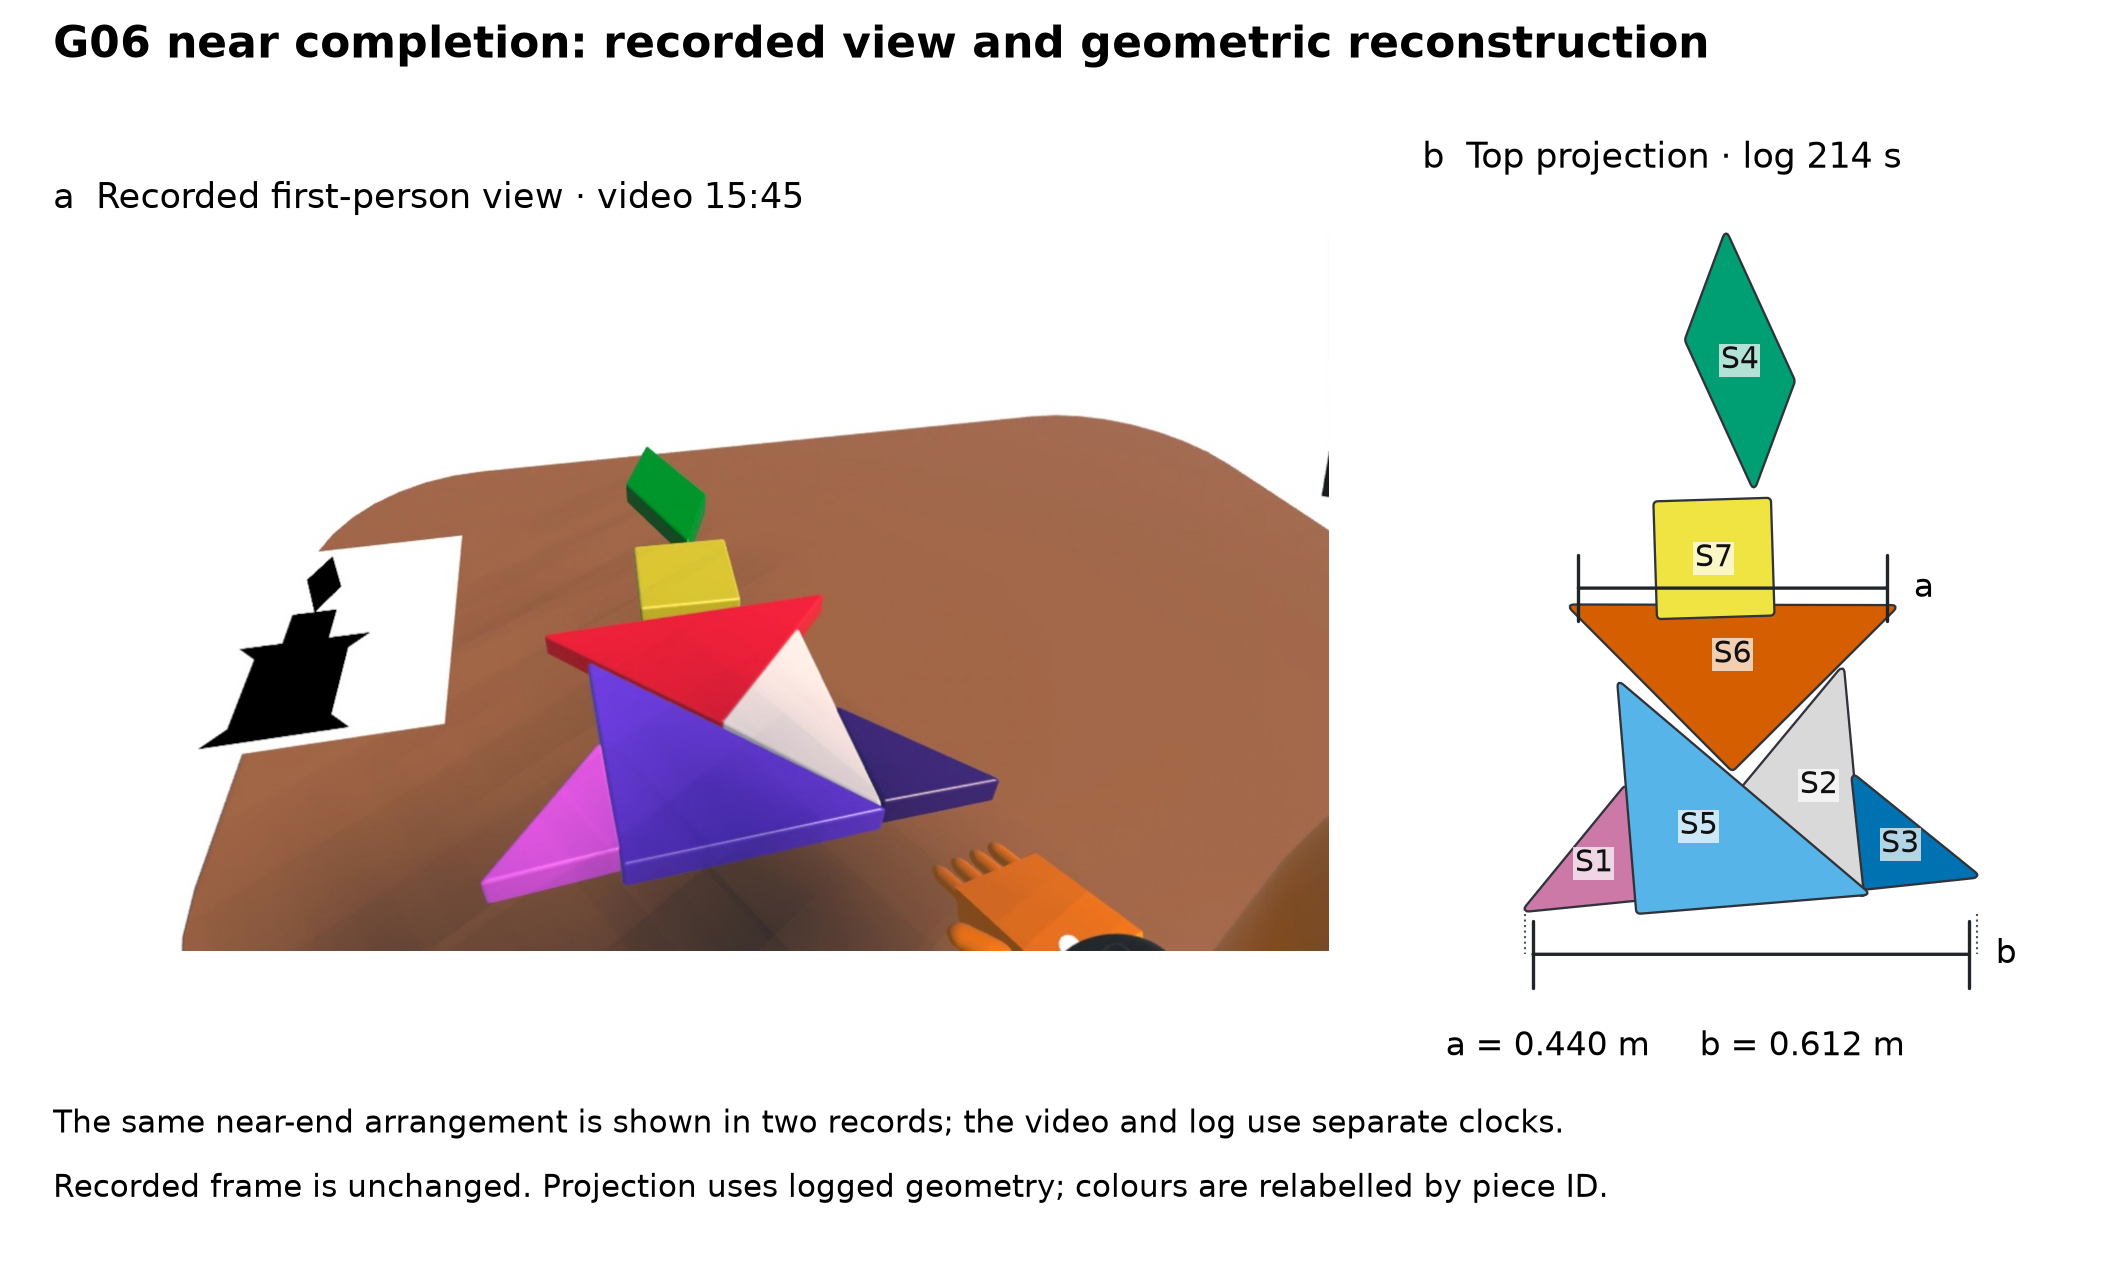
\includegraphics[width=\linewidth,height=153mm,keepaspectratio]{assets/figures/fig03_g06_recorded_view_and_geometry.png}
\captionof{figure}[The near-end G06 arrangement in a recorded first-person frame at 15:45 (left) and a reconstruction at 214 active-task...]{The near-end G06 arrangement in a recorded first-person frame at 15:45 (left) and a reconstruction at 214 active-task seconds (right). These are independent video and log clocks, showing the same near-end arrangement rather than frame-exact synchronisation. The reconstruction uses colours assigned by piece ID. Dimension a is the upper large triangle's longest projected chord; b is the lower-piece span along that direction. This is an analytical comparison, not an in-task switch to overhead viewing. [\hyperlink{src:D14}{D14}, \hyperlink{src:D16}{D16}]}\label{fig:5-2}
\par\endgroup
\end{figureunit}



\begin{samepage}
The recorded first-person view and the log-based reconstruction show the near-end arrangement on their respective time bases. The reconstruction makes the unequal spans directly inspectable. In an oblique view, the apparent lengths and angles depend on viewing direction and distance; a perpendicular orthographic view preserves the shape of the planar arrangement. The case therefore connects an observed judgment during collaboration with a specific geometric mismatch. Section~\ref{sec:6-1} considers what this relationship means for viewpoint design.
\par\end{samepage}

\begin{figureunit}{5-3}
\par\begingroup
\centering
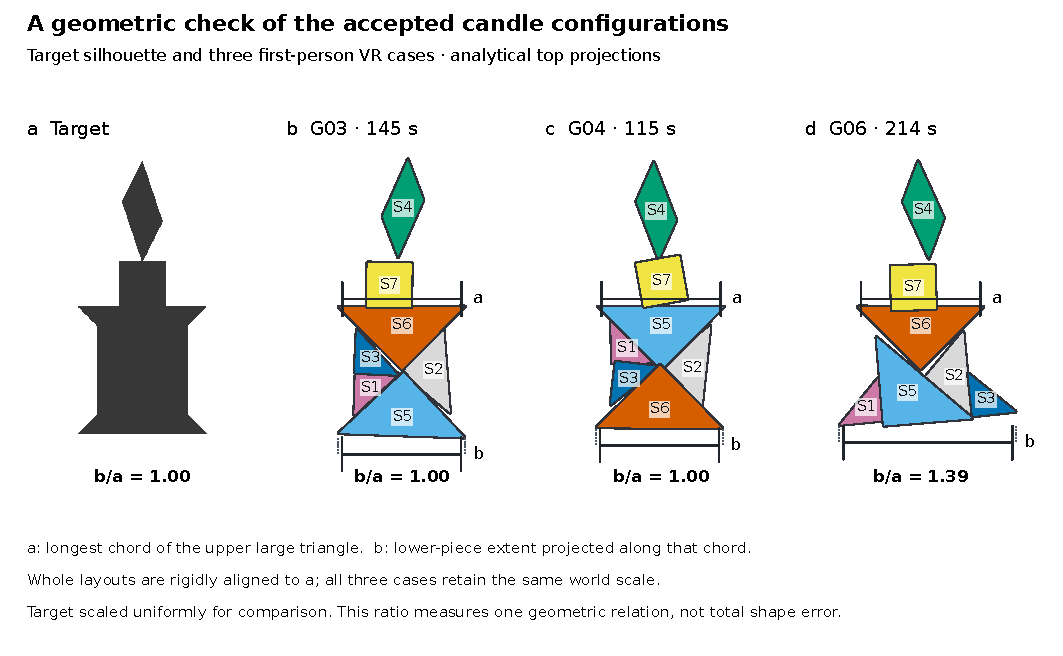
\includegraphics[width=\linewidth,height=153mm,keepaspectratio]{assets/figures/fig02_candle_geometry_comparison.pdf}
\captionof{figure}[Target silhouette and three first-person VR configurations.]{Target silhouette and three first-person VR configurations. Entire layouts are translated and rigidly rotated to align a; individual piece relations and world scale are preserved. The lower span b uses one large triangle in G03 and G04, and S1/S5/S3 in G06. The displayed span ratios are 1.00, 1.00 and 1.39, respectively. The target silhouette is scaled uniformly for display. This ratio measures one width relation, not total shape error. Rounded mesh corners and thickness are retained. [\hyperlink{src:D16}{D16}, \hyperlink{src:D06}{D06}, \hyperlink{src:D08}{D08}, \hyperlink{src:D14}{D14}]}\label{fig:5-3}
\par\endgroup
\end{figureunit}




The two pieces of evidence address complementary questions. The condition-level process records identify where the near-complete shape problems occurred. The G06 reconstruction identifies a measurable mismatch in a particular accepted construction. The fixed sequence, different target patterns and prototype versions remain part of the condition comparison; the examples establish the practical relevance of geometric presentation within the studied tasks.


\section{Expressing ideas and continuing shared constructions}\label{sec:5-2}

Participants expressed local ideas through placements that their partners could inspect, continue or change. Who advanced a part could change during the round, and both participants could return to an arrangement when the remaining pieces did not fit. The process records and action logs trace how these contributions connected within the shared task.

\begin{samepage}
In G06's first-person candle, the initial body-and-top arrangement became a shared reconstruction problem when the medium triangle remained unused. Both participants subsequently manipulated the body. The logged sequence in Figure~\ref{fig:5-4} shows who handled each piece and when. It makes the move from separate local work to repeated intervention in the same set of pieces inspectable. The six reconstructed states in Figure~\ref{fig:5-1} show what those actions produced. Read together, the two figures connect a change in work organisation to the changing configuration, rather than treating all grabs as equivalent contributions.
\par\end{samepage}

\begin{figureunit}{5-4}
\par\begingroup
\centering
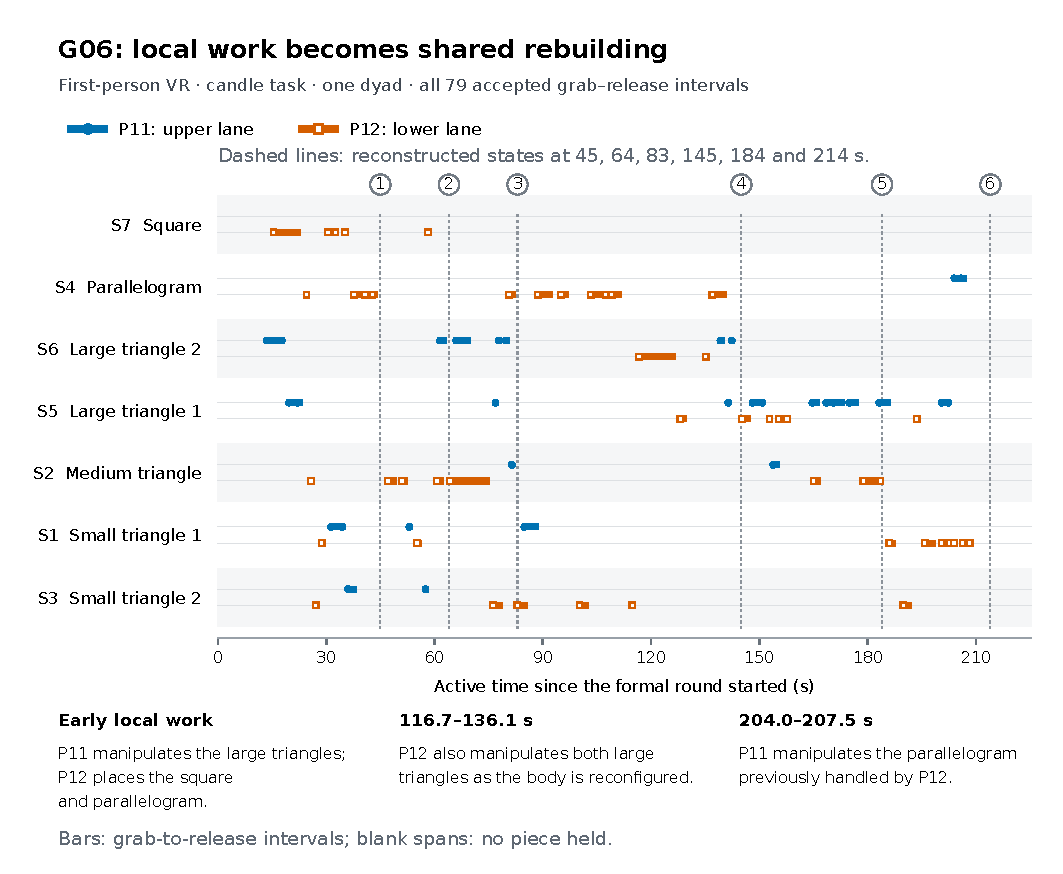
\includegraphics[width=\linewidth,height=132mm,keepaspectratio]{assets/figures/F3_G06_action_timeline.pdf}
\captionof{figure}[All 79 logged manipulation intervals in G06's first-person candle round.]{All 79 logged manipulation intervals in G06's first-person candle round. P11 is the upper lane and P12 the lower lane for each piece. A segment runs from accepted grab to release; its marker identifies the grab. Vertical guides match the six states in Figure~\ref{fig:5-1}. Later actions cross the initial body/top division: P12 handles both large triangles and P11 handles the parallelogram. Object control does not measure idea ownership or relative contribution. Participant identities follow the recording-position mapping and checked endpoint alignment. [\hyperlink{src:D14}{D14}]}\label{fig:5-4}
\par\endgroup
\end{figureunit}

\begin{samepage}
The change is visible at piece level. P11 first grabbed large triangle S6 at 13.58 active seconds, while P12 handled square S7 from 15.40 to 22.87 seconds. Later, P12 manipulated S6 from 116.67 to 126.75 seconds and the other large triangle, S5, from 128.07 to 129.79 seconds. Between 145.14 and 158.71 seconds, S5 was manipulated in sequence by P12, P11 and P12. Near the end, P11 manipulated the parallelogram S4 in two intervals, 204.03--204.90 and 205.89--207.47 seconds, after P12 had handled it earlier. These changes show the initially separate work on the body and top becoming repeated manipulation of the same pieces by both partners. [\hyperlink{src:D14}{D14}]
\par\end{samepage}



G03's candle developed through a different sequence. P05 proposed using two small triangles for the flame, while P06 used the parallelogram for that part. P06 invited P05 to move to the same side of the table, and P05 did so. The pair still pursued different flame constructions. At approximately 03:06 in P05's recording, P05 dismantled the two-small-triangle arrangement and used those pieces for the base. P06 later continued the solution, and the candle was completed. The source records show overlapping local attempts followed by a reallocation of both pieces and work. Their common viewing position preceded the resolution of the different construction ideas. [\hyperlink{src:D06}{D06}]



\begin{samepage}
The G03 logs also provide a direct trace of self-revision followed by partner continuation (Figure~\ref{fig:5-5}). By 52 active seconds, P05 had brought small triangles S1 and S3 together. P05 grabbed them again at 67.38 and 69.33 seconds; the 73-second reconstruction shows them separated. P06 subsequently grabbed S3 at 93.56 seconds and S1 at 96.29 seconds. The 99-second state shows the resulting changes. The same pieces therefore passed from one person's local arrangement, through that person's revision, to manipulation by the partner. The endpoint-to-participant mapping was checked against three visible grabs in the recording. The video account supplies the interpretations of flame and base; its reported event and the selected log snapshots are shown at their respective recorded times. [\hyperlink{src:D06}{D06}]
\par\end{samepage}

\begin{figureunit}{5-5}
\par\begingroup
\centering
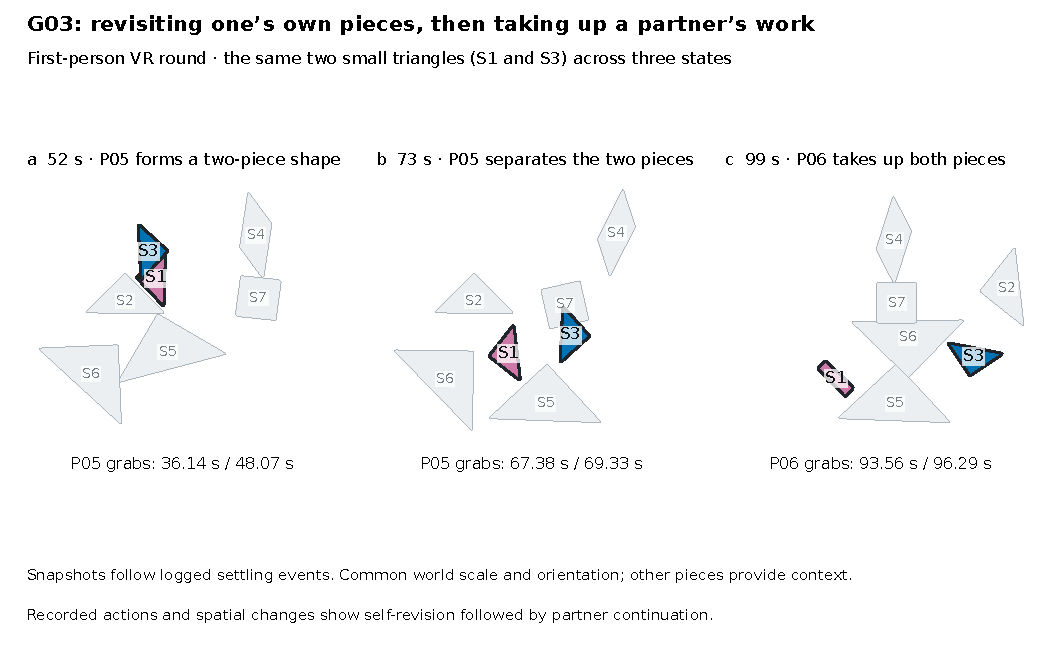
\includegraphics[width=\linewidth,height=100mm,keepaspectratio]{assets/figures/fig04_g03_self_revision_and_continuation.pdf}
\captionof{figure}[G03 configurations at 52, 73 and 99 active seconds, with the same scale and orientation.]{G03 configurations at 52, 73 and 99 active seconds, with the same scale and orientation. S1 and S3 are highlighted; other pieces show context. P05 brings them together, later separates them, and P06 subsequently operates on both. The snapshots follow settling events at 51.522, 72.518 and 98.699 seconds. S1 is nearly edge-on in the last projection because its recorded three-dimensional pose is retained. These selected states show self-revision followed by partner continuation; intermediate actions remain in the source event list. [\hyperlink{src:D06}{D06}]}\label{fig:5-5}
\par\endgroup
\end{figureunit}

In G01's physical direct-view chicken task, P02 questioned P01's proposed use of a large triangle for the back at approximately 00:34. P01 continued the attempt. Around 01:05, P02 began trying the alternative by fitting the medium and large triangles together. The researcher reported that P01 then accepted this arrangement and moved to other parts around 01:20. At 01:25, P01 proposed using a small triangle for the head; P02 added the square beneath it at 01:27, and P01 straightened it. The sequence moved from disagreement about a local part to an enacted alternative, followed by work on the next part. [\hyperlink{src:D01}{D01}]

\begin{figureunit}{5-6}
In G06's physical overhead goose task, P12 initially placed the square as the head. P11 added a small triangle and the parallelogram for the mouth and neck. At approximately 00:33, P11 tried to establish the body's large-triangle arrangement without resolving it. P12 continued from the existing neck by adding a small triangle at 00:53. P11 placed the medium triangle against it at 01:02. From approximately 01:11, both participants placed the remaining large triangles, and the researcher recorded successful completion at 01:20. During the subsequent reference check, their solution had a different internal partition: the head region combined the square and a small triangle, while the reference used the medium triangle and a small triangle, with the other combination in the corresponding body region. Figure~\ref{fig:5-6} shows the successive additions and the later reference check. [\hyperlink{src:D12}{D12}]

\par\begingroup
\centering
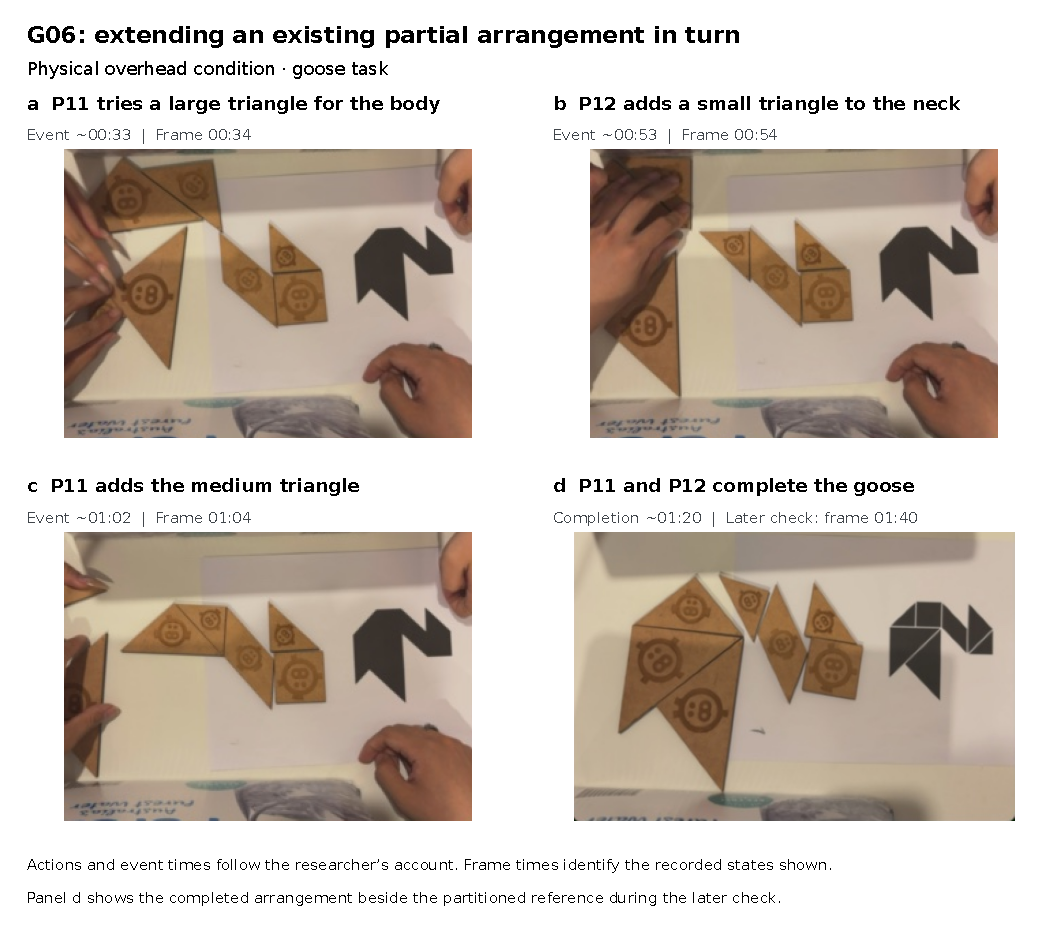
\includegraphics[width=\linewidth,height=115mm,keepaspectratio]{assets/figures/fig07_g06_goose_continuation.pdf}
\captionof{figure}[G06 extending a partial goose arrangement in the physical overhead condition.]{G06 extending a partial goose arrangement in the physical overhead condition. The researcher's process account records P11 trying a large triangle for the body (a, approximately 00:33), P12 adding a small triangle to the existing neck (b, 00:53), and P11 continuing with the medium triangle (c, 01:02). Both participants then placed the remaining large triangles and completed the goose at approximately 01:20. Panel d shows the later reference check at 01:40. The completed arrangement uses a different internal partition from the reference: the square and medium triangle occur in different regions, each paired with a small triangle. Event times and actor attribution follow the researcher's account; frame times identify the displayed video images. [\hyperlink{src:D12}{D12}]}\label{fig:5-6}
\par\endgroup
\end{figureunit}



\begin{samepage}
In the G06 interview, one participant described treating the partner's not removing their placed pieces as a sign that the partner understood what they were doing. In response to a discussion of the task's division into parts, the transcript also records a participant describing a division of work that had not been explicitly stated. These statements are paraphrased from the group transcript; individual speaker attribution was not resolved. [\hyperlink{src:D13}{D13}]
\par\end{samepage}

Complementary work could also emerge through a proposal that other placements then extended. In G04's first-person candle, P08 explained at approximately 07:10 that the two large triangles would form four corners and that the sides could then be filled. At approximately 07:33, P08 placed the medium triangle while P07 placed the square. P07 placed the parallelogram around 07:35, and each participant placed a small triangle around 07:40. The proposal and subsequent placements show how an emerging construction supported compatible actions by both people. [\hyperlink{src:D08}{D08}]

The shared-overhead rounds show how local control difficulties could change who performed a step. In G05, the process notes describe one participant mainly suggesting placements while the other manipulated the pieces. The main manipulator later requested help when a piece was out of reach. G06 likewise included assistance after a technical interruption and restart. These were freely organised responses to the immediate task, rather than assigned director and operator roles. A participant could move from proposing a placement to making it, or from continuing another part to helping with a blocked action. [\hyperlink{src:D11}{D11}, \hyperlink{src:D15}{D15}]

Across these cases, a proposal or partial arrangement provided a next step for either partner. Separate activity, continuation and joint reconstruction occurred within the same round, connected through the shared pieces and the developing shape.

\section{Preserving a partner's construction and revising one's own}\label{sec:5-3}

Several episodes distinguish the person who initially constructed a part from the person who later changed it. A partner could tidy or continue an existing arrangement while its original builder subsequently reopened it. The clearest instances include a correct partial construction that was changed into an incorrect one. Table~\ref{tab:5-2} brings these episodes together with cases of direct partner revision.

\par\addvspace{8pt}
\noindent\begin{minipage}{\linewidth}
\begingroup
\centering
\setstretch{1}
\fontsize{10}{12.3}\selectfont
\setlength{\tabcolsep}{2.2pt}
\renewcommand{\arraystretch}{1.18}
\captionof{table}[Selected trajectories of partial solutions.]{Selected trajectories of partial solutions. Correctness labels follow the researcher's process reports; each row is an episode, not a frequency estimate.}\label{tab:5-2}
\begin{tabular}{@{}>{\raggedright\arraybackslash}p{23.075mm}>{\raggedright\arraybackslash}p{68.301mm}>{\raggedright\arraybackslash}p{65.532mm}@{}}
\toprule
\textbf{Case} & \textbf{Later action} & \textbf{Result or role} \\
\midrule
G01 R02 & P01 builds; P02 tidies; P01 changes the arrangement. & Correct head/neck changed into an incorrect arrangement. \\
\addlinespace[3pt]
G03 R03 & P05 dismantles P05's small-triangle arrangement; work continues. & Pieces reassigned; the log also traces self-revision then partner continuation. \\
\addlinespace[3pt]
G04 R01 & P08's approach is revisited; researcher then confirms its earlier correctness. & P08's useful idea is reopened; task eventually abandoned. \\
\addlinespace[3pt]
G05 R03 & Original builder changes the parallelogram's role; partner later restores it. & Self-revision followed by partner repair. \\
\addlinespace[3pt]
G03 R01 & P06 changes P05's horse head while P05 continues the body. & Direct partner intervention. \\
\addlinespace[3pt]
G01 R01 & Both partners repeatedly adjust the same large triangle. & Mutual revision during a disagreement. \\
\bottomrule
\end{tabular}
\par\endgroup
\end{minipage}\par\addvspace{8pt}

\begin{samepage}
In G01's physical-overhead goose task, P01 placed the small triangle and parallelogram together at approximately 04:38, producing the head and neck that the researcher judged correct. At approximately 06:01, P02 tidied these two pieces. At approximately 06:26, P01 rotated the parallelogram and joined it to a large triangle, changing to an incorrect arrangement. Figure~\ref{fig:5-7} follows this sequence in the video. The decisive change was made by the person who had built the correct local solution, after the partner had adjusted that existing solution. [\hyperlink{src:D03}{D03}]
\par\end{samepage}

\begin{figureunit}{5-7}
\par\begingroup
\centering
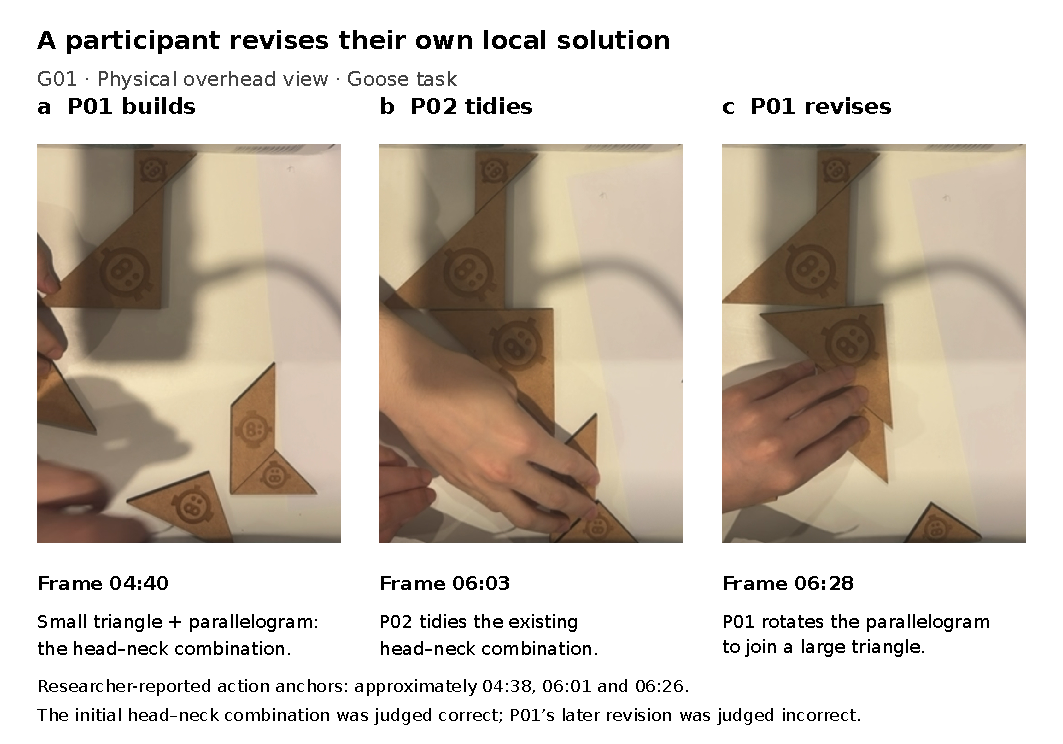
\includegraphics[width=\linewidth,height=96mm,keepaspectratio]{assets/figures/F4_self_revision.pdf}
\captionof{figure}[G01's physical-overhead goose task.]{G01's physical-overhead goose task. P01 builds the head and neck; P02 tidies the combination; P01 later rotates the parallelogram to join a large triangle. The researcher's video-review record judges the first local arrangement correct and the later revision incorrect. Frames at 04:40, 06:03 and 06:28 are close to reported action anchors at 04:38, 06:01 and 06:26. Crops remove call-interface identifiers and preserve the original projection. Hands occlude some edges; the middle still does not independently establish that P02 changed only alignment. [\hyperlink{src:D03}{D03}]}\label{fig:5-7}
\par\endgroup
\end{figureunit}



Here, the partner's intervention did not itself account for the loss of the correct head-and-neck arrangement. The reported sequence places P02's tidying before P01's explicit structural change. The event shows how a useful partial solution can be reopened by its original builder during a joint task.

G04's physical-direct task provides a second instance of a useful idea being reopened by its own builder. At approximately 05:30, P08 developed an approach that the researcher regarded as correct, then changed it again around 06:13. After this change, the researcher pointed out that the preceding approach had been correct. The task was eventually abandoned. This episode shows a useful construction being reopened by its own builder. [\hyperlink{src:D07}{D07}]

G03's first-person candle gives a different outcome for self-revision. P05 dismantled the small-triangle flame that P05 had made and repurposed its pieces for the base. Here, changing one's own work contributed to resolving the conflict between the two initial approaches. The contrast with G01 is instructive: self-revision can support progress or remove a correct part. Its consequence depends on the relationship between the revised part, the remaining pieces and the developing whole. [\hyperlink{src:D06}{D06}] The pose sequence in Figure~\ref{fig:5-5} adds a trace of one logged participant rearranging their own two-piece construction before the other participant handled those pieces.

In G05's first-person chair, the process notes describe P09 moving away from an almost-correct arrangement and changing the parallelogram's role, while P10 questioned the change. P10 later returned it to the backrest. This sequence joins self-revision to partner repair: the original builder's reconsideration did not simply end the attempt, because the partner later acted on the same part. The description of the earlier arrangement as almost correct comes from the process report. [\hyperlink{src:D10}{D10}]

Partners also changed each other's work. In G03's physical-direct horse task, P06 objected to P05's head construction and changed it while P05 continued with the body. In G01's physical-direct task, both partners repeatedly adjusted the same large triangle during a short disagreement around 01:36--01:40. These episodes show direct intervention in an existing local construction. They make the distinction between preservation, tidying and structural revision necessary when describing how a partner responded. [\hyperlink{src:D05}{D05}, \hyperlink{src:D02}{D02}]

G05 adds a related verbal sequence. P09 questioned the idea that the goose's body required large triangles and revised the idea while P10 gave no response during that interval. This is recorded as self-correction of a proposal. It complements the manipulation cases by showing that an apparent change in the pair's direction can originate in one person's reconsideration, even when both people are present. [\hyperlink{src:D09}{D09}]

G06's candle logs also show retention during reconstruction. No later pose change was recorded for the square after it settled at 59.79 active seconds, or for the new red large-triangle placement after 143.33 seconds, while other pieces continued to be manipulated. These retained placements and the surrounding rebuilding occurred within the same sequence. The statement concerns the recorded geometry at the logging resolution described in Section~\ref{sec:4-4}. [\hyperlink{src:D14}{D14}]

The finding concerns the trajectories of existing partial solutions: who develops them, who keeps them available, and who changes their structure. These trajectories reveal a form of coordination that a final picture alone would miss. A retained piece may carry earlier work into the next step, while a new manipulation can reopen a decision that had appeared settled. The video records establish the local interaction; where available, the pose logs make the change of operator and geometry directly traceable.


\section{Questionnaire perspectives on communication and control}\label{sec:5-4}

\begin{figureunit}{5-8}
The questionnaire adds a participant-level account of placement communication, progress awareness, piece control and joint solving (Figure~\ref{fig:5-8}). Ratings differed across these aspects. From first-person VR (R03) to shared overhead VR (R04), three participants rated explaining an intended placement more highly, eight gave the same rating and one gave a lower rating. Movement and rotation each received lower ratings from five participants, the same ratings from six and a higher rating from one. Communicating a placement and controlling a piece were therefore distinct aspects of the reported experience.

\par\begingroup
\centering
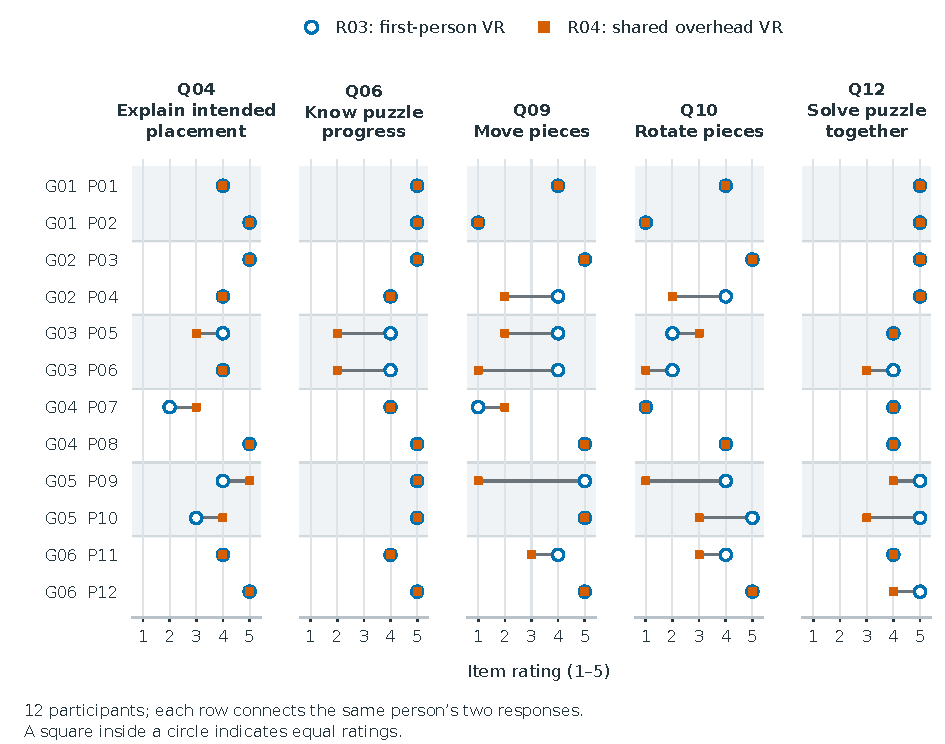
\includegraphics[width=\linewidth,height=120mm,keepaspectratio]{assets/figures/Figure5_8_VR_item_ratings.pdf}
\captionof{figure}[Paired ratings for five questionnaire items in first-person VR (R03) and shared overhead VR (R04).]{Paired ratings for five questionnaire items in first-person VR (R03) and shared overhead VR (R04). Each row is one participant; circles and squares show the two raw ratings, connected within that participant. A square inside a circle indicates equal ratings. All 12 participants have both responses for these items (24 VR questionnaires from the confirmed 48-response dataset). Q04 concerns explaining an intended placement, Q06 knowing puzzle progress, Q09 moving a piece to an intended location, Q10 rotating it to an intended orientation, and Q12 feeling that the puzzle was solved together. Ratings use the full 1--5 scale; no combined score is calculated. The rounds occurred in a fixed order with different target patterns. G01 used the earlier target presentation and G02--G06 the revised version. G02 ratings describe the original session; the relationship to the later recordings is explained in Section~\ref{sec:4-1}.}\label{fig:5-8}
\par\endgroup
\end{figureunit}

The differences are visible within dyads. In G05, both participants rated explaining a placement more highly in R04, while their ratings of solving together fell from 5 to 4 and from 5 to 3. P09 also rated moving pieces from 5 to 1 and rotating them from 4 to 1. In G04, both participants rated solving together at 4 in both rounds, although P07 rated rotation at 1 and P08 at 4. The questionnaire therefore supplements the action evidence by showing that a sense of working together can coexist with very different experiences of control. The comparisons describe sessions with a fixed condition order and different target patterns. G01 used the earlier target presentation; G02--G06 used the revised version.




\section{Connecting viewing conditions to the collaborative process}\label{sec:5-5}

The three findings connect through the evolving construction. Participants used the visible arrangement to decide where to work, which pieces to use and what to keep or revise. In G06, the initial division between body and top was followed by shared reconstruction around an apparently plausible candle. The partners completed the seven-piece arrangement and accepted it, while the later reconstruction confirmed the researcher's observation of a proportion problem. Viewing, work organisation and outcome judgment were therefore present within the same sequence.

The other cases show different paths through that relationship. G01 rejected a first-person candidate when a substitution failed to align. G05 continued working after a partner questioned the proportions. G03 reorganised overlapping local attempts by reallocating its small triangles. In the physical-overhead G01 case, a correct part was kept and tidied before its original builder changed it. These outcomes locate the contribution of an overhead view alongside the continuing work of interpreting, revising and coordinating a solution.

For this planar task, the overhead view's geometric advantage matters because shape and proportion are resources used throughout collaboration. The results support evaluating that view through the actual actions it accompanies: how participants establish a candidate, continue one another's work, notice a conflict and decide what to change. The action records also reveal why viewing the final arrangement alone provides an incomplete account of collaboration. The same ending can arise through different divisions of work, and a useful partial solution can be lost before the ending is reached.

